\documentclass[rgb]{beamer}

\usepackage[english]{babel}
\usepackage[utf8]{inputenc}
\usepackage{xcolor}
\usepackage{listings}
\usepackage{adjustbox}
\usepackage{amsmath}
\usepackage{multirow}
\usepackage[linewidth=1pt]{mdframed}

% Graphics
\usepackage{graphicx}

\usepackage{tikz}
\usetikzlibrary{calc,shapes.multipart,chains,arrows}

% Font
\usepackage{paratype}
\setbeamerfont{frametitle}{family=\bf}

% Beamer theme settings
\usecolortheme{seagull}
\setbeamertemplate{itemize item}{\raisebox{0.8mm}{\rule{1.8mm}{1.2mm}}}
\usenavigationsymbolstemplate{} % no navigation buttons

\usepackage{listings}

% Define Language
\lstdefinelanguage{fsharp}
{
  % list of keywords
  morekeywords={
    and,
    do,
    else,
    exception,
    for,
    fun,
    function,
    if,
    in,
    let,
    match,
    module,
    mutable,
    open,
    of,
    rec,
    then,
    try,
    type,
    unsafe,
    use,
    val,
    when,
    while,
    with,
  },
  sensitive=true, % keywords are not case-sensitive
  morecomment=[l]{//}, % l is for line comment
%  otherkeywords={>,<,=,<=,>=,!,*,/,-,+,|,&,||,&&,==,=>},
  morestring=[b]" % defines that strings are enclosed in double quotes
}

% Define Colors
\usepackage{color}
\definecolor{eclipseBlue}{RGB}{42,0.0,255}
\definecolor{eclipseGreen}{RGB}{63,127,95}
\definecolor{eclipsePurple}{RGB}{127,0,85}

\newcommand{\fop}[1]{\mbox{\ttfamily\color{eclipseBlue}#1}}
\newcommand{\fw}[1]{\mbox{\ttfamily\bfseries\color{eclipsePurple}#1}}

% Set Language
\lstset{
  language={fsharp},
  basicstyle=\ttfamily, % Global Code Style
  captionpos=b, % Position of the Caption (t for top, b for bottom)
  extendedchars=true, % Allows 256 instead of 128 ASCII characters
  tabsize=2, % number of spaces indented when discovering a tab
  columns=fixed, % make all characters equal width
  keepspaces=true, % does not ignore spaces to fit width, convert tabs to spaces
  showstringspaces=false, % lets spaces in strings appear as real spaces
  breaklines=true, % wrap lines if they don't fit
  frame=trbl, % draw a frame at the top, right, left and bottom of the listing
  frameround=tttt, % make the frame round at all four corners
  framesep=4pt, % quarter circle size of the round corners
  numbers=left, % show line numbers at the left
  numberstyle=\small\ttfamily, % style of the line numbers
  commentstyle=\slshape\bfseries\color{eclipseGreen}, % style of comments
  keywordstyle=\bfseries\color{eclipsePurple}, % style of keywords
  stringstyle=\color{eclipseBlue}, % style of strings
  emph=[1] {
    false,
    true,
    Set,
    Map,
    List,
    ImgUtil,
    Pegs,
    String,
    Array,
    Array2D
  },
  emphstyle=[1]{\color{eclipseBlue}},
  moredelim=**[is][\color{red}]{@@}{@@}
}

\newcommand{\theyear}{2020}
\newcommand{\sem}[1]{[\![#1]\!]}
\newcommand{\seme}[1]{\sem{#1}\varepsilon}
\newcommand{\semzero}[1]{\sem{#1}_0}

\newcommand{\emptymap}{\{\}}
\newcommand{\fracc}[2]{\begin{eqnarray} \frac{\begin{array}{c} #1
    \end{array}}{\begin{array}{c} #2 \end{array}} \end{eqnarray}}
\newcommand{\sembox}[1]{\hfill \normalfont \mbox{\fbox{\(#1\)}}}
\newcommand{\sempart}[2]{\subsubsection*{\rm\em #1 \sembox{#2}}}
\newcommand{\axiom}[1]{\begin{eqnarray} \begin{array}{c} #1 \end{array} \end{eqnarray}}
\newcommand{\fraccn}[2]{\refstepcounter{equation}\mbox{$\frac{\begin{array}{c} #1 \end{array}}{\begin{array}{c} #2 \end{array}}$}~(\arabic{equation})}
\newcommand{\fraccc}[2]{\mbox{$\frac{\begin{array}{c} #1 \end{array}}{\begin{array}{c} #2 \end{array}}$}}
\newcommand{\onepart}[1]{\noindent\hfill#1\hfill~\vspace{2mm}}
\newcommand{\twopart}[2]{\noindent\hfill#1\hfill#2\hfill~\vspace{2mm}}
\newcommand{\threepart}[3]{\noindent\hfill#1\hfill#2\hfill#3\hfill~\vspace{2mm}}
%\newcommand{\axiomm}[1]{\refstepcounter{equation}\mbox{$\begin{array}{c} #1 \end{array}$}~(\arabic{equation})}
\newcommand{\axiomm}[1]{$\begin{array}{c} #1 \end{array}$}
%\newcommand{\ar}[1]{\stackrel{#1}{\longrightarrow}}
\newcommand{\vd}{\vdash}
\newcommand{\Ran}{{\rm Ran}}
\newcommand{\Dom}{{\rm Dom}}
\newcommand{\kw}[1]{\texttt{#1}}
\newcommand{\id}[1]{\mbox{\it{#1}}}
\newcommand{\rarr}{\rightarrow}
\newcommand{\eval}{\rarr}
\newcommand{\evals}{\leadsto}
\newcommand{\larr}{\leftarrow}

\newcommand{\head}[1]{\vspace{3mm} \textbf{\normalsize #1}}
\newcommand{\headsp}[1]{\head{#1}\vspace{1ex}}
\newcommand{\size}{\ensuremath{\mathrm{size}}}
\renewcommand{\log}{\ensuremath{\mathrm{log}}}

\newcommand{\setallthemecolors}[1]{%
\setbeamercolor*{palette primary}{use=structure,fg=white,bg=#1}%
\setbeamercolor*{palette secondary}{use=structure,fg=white,bg=#1}%
\setbeamercolor*{palette tertiary}{use=structure,fg=white,bg=#1}}

\definecolor{black}{RGB}{0,0,0}
\definecolor{maroon}{RGB}{128,0,0}
\definecolor{olive}{RGB}{128,128,0}
\definecolor{green}{RGB}{0,128,0}
\definecolor{purple}{RGB}{128,0,128}
\definecolor{teal}{RGB}{0,128,128}
\definecolor{darkteal}{RGB}{0,92,92}
\definecolor{navy}{RGB}{0,0,128}
\definecolor{gray}{RGB}{128,128,128}
\definecolor{darkgray}{RGB}{60,60,60}
\definecolor{darkred}{RGB}{139,0,0}

%palette

% #173F5F (dark blue)
\definecolor{darkblue}{RGB}{23,63,95}
% #20639B (blue)
\definecolor{blue}{RGB}{32,99,155}
% #3CAEA3 (green)
\definecolor{magenta}{RGB}{60,174,163}
% #F6D55C (yellow)
\definecolor{yellow}{RGB}{246,213,92}
% #ED553B (red)
\definecolor{red}{RGB}{237,85,59}


\usecolortheme{whale}
\useoutertheme{infolines}
\useinnertheme{rectangles}

\newcommand{\popsettitle}[2]{%
\setallthemecolors{#1}%
\newcommand{\popemne}{#2}%
\title{Programmering og Problemløsning}%
\subtitle{#2}%
\author{Martin Elsman}%
\date{}%
\institute[DIKU]{Datalogisk Institut, Københavns Universitet (DIKU)}}

\newcommand{\popmaketitleframe}{%
  \frame{\titlepage%
   \vspace{-15mm}%
   \par\noindent\rule{\textwidth}{0.4pt}%

   \vspace{4mm}%
   \tableofcontents%
   \vspace{-4mm}%
   \par\noindent\rule{\textwidth}{0.4pt}%
  }%
  \section*{\popemne}%
}


\popsettitle{purple}{Typer og Mønstergenkendelse (Del 4; Recap)}  % see ../util.tex for colors

\begin{document}

\newcommand{\fboxred}[1]{\color{darkred}\fbox{#1}}
\popmaketitleframe

%%%%%%%%%%%%%%%%%%%%%%%%%%%%%%%%%%%%%%%%%%%%%%%%
%\subsection{Introduktion}
%%%%%%%%%%%%%%%%%%%%%%%%%%%%%%%%%%%%%%%%%%%%%%%%

%% Recap:
%   typeforkortelser
%   produkttyper (tupler og records)
%   sum-typer
%   generiske typer
%   abstrakte typer
%   mønstergenkendelse (pattern matching)

\subsection{Recap}

\begin{frame}[fragile]
\begin{footnotesize}

  \headsp{Simple sum-typer (enumerations)}
  \vspace{1ex}

  \head{Eksempler:}
\begin{lstlisting}[numbers=none,frame=none,mathescape]
  type country = DK | UK | DE | SE | NO
  type currency = DKK | EUR | USD | CHF | GBP
  type direction = North | South | East | West
\end{lstlisting}

  \vspace{1ex}
  \head{Pattern-matching:}

\begin{lstlisting}[numbers=none,frame=none,mathescape]
  let opposite (dir:direction) : direction =
    match dir with
      | North -> South    // A constructor can appear
      | South -> North    // both as a pattern and as
      | East -> West      // an expression (just as
      | West -> East      // integers can)
\end{lstlisting}

\head{Bemærk:}
\begin{itemize}
\item Det kan være en fordel at benytte sig af simple sum-typer i
  stedet for f.eks. streng- eller heltals-repræsentationer af data.
\end{itemize}

\end{footnotesize}
\end{frame}

\begin{frame}[fragile]
\begin{footnotesize}

  \headsp{Sum-typer med argument-bærende konstruktører}

\begin{lstlisting}[numbers=none,frame=none,mathescape]
  type object = Pnt | Circ of float | Rect of float * float
\end{lstlisting}

  \vspace{1ex}
  \head{Pattern-matching er nu mulig:}
\begin{lstlisting}[numbers=none,frame=none,mathescape]
  let rec area (obj:object) : float =
    match obj with
    | Pnt -> 0.0
    | Circ r -> System.Math.PI * r * r
    | Rect (a,b) -> a * b
\end{lstlisting}

  \vspace{1ex}

\head{Bemærk:}
\begin{itemize}
\item Det er ikke et krav at alle konstruktører tager argumenter; \lstinline{Pnt} tager ikke et argument.
\item Konstruktører der tager argumenter virker som funktioner i udtryk; f.eks. har \lstinline{Circ} typen \lstinline{float -> object}.
\end{itemize}

\end{footnotesize}
\end{frame}

\begin{frame}[fragile]
\begin{footnotesize}

  \headsp{Typer kan være type-generiske}

  Type-definitioner kan være \emph{generiske} ved at være
  parameteriserede over andre typer, såsom \lstinline{option}-typen:

\begin{lstlisting}[numbers=none,frame=none,mathescape]
  type 'a option = None | Some of 'a
\end{lstlisting}

  \vspace{1ex}
  \headsp{Vi kan nu skrive generisk (genbrugelig) kode:}
\begin{lstlisting}[numbers=none,frame=none,mathescape]
  let valOf (def:'a) (obj:'a option) : 'a =
    match obj with
    | None -> def
    | Some v -> v
\end{lstlisting}

  \headsp{Vi kan nemt læse hvad følgende funktion gør (fra modulet \lstinline{List}):}

\begin{lstlisting}[numbers=none,frame=none,mathescape]
  val tryFind : ('a -> bool) -> 'a list -> 'a option
\end{lstlisting}

\end{footnotesize}
\end{frame}

\begin{frame}[fragile]
\begin{footnotesize}

  \head{Sum-typer er et meget kraftigt redskab}
  \vspace{1ex}

  Sum-typer åbner op for en lang række muligheder:
  \vspace{1ex}
  \begin{itemize}
  \item Sum-typer kan moduleres med produkter (tupler), men giver
    mulighed for en mere præcis definition af data-sammenhænge.
  \vspace{1ex}
  \item Sum-typer baner vejen for let at definere såkaldte ``embeddede''
    domain-specifikke sprog (EDSLs).
  \vspace{1ex}
  \item Sammen med pattern-matching giver sum-typer beriget kontrol
    over at alle kode-tilfælde er håndteret (jvf. \lstinline{area} funktionen).
  \end{itemize}

  \vspace{1ex}

  \headsp{Rekursivt-definerede sum-typer}
  \begin{itemize}
  \item Lister kan (som nævnt) forstås som en generisk rekursivt-defineret sum-type med to konstruktører (\lstinline{[]} og \lstinline{::}).
\begin{lstlisting}[numbers=none,frame=none,mathescape]
  type 'a list = [] | (::) of 'a * 'a list
\end{lstlisting}
  \item Vi skal senere se hvorledes vi også kan definere mere avancerede generiske data-strukturer, såsom træer, ved hjælp af generiske rekursive sum-typer.
  \end{itemize}

\end{footnotesize}
\end{frame}

\begin{frame}[fragile]
\begin{footnotesize}
  \headsp{Nogle spørgsmål}

\vspace{2mm}

  \begin{itemize}
  \item Hvordan får man værdien af en \lstinline{option} type (og hvad gør man hvis værdien kan være \lstinline{None})?
\vspace{4mm}
  \item Hvordan ved man om man skal bruge pattern matching eller \lstinline{if}-expressions?
\vspace{4mm}
  \item \rule{.9\textwidth}{0.4pt}
\vspace{4mm}
  \item \rule{.9\textwidth}{0.4pt}
  \end{itemize}

\end{footnotesize}
\end{frame}


\subsection{Typer som problemløsningsværktøj}

\begin{frame}[fragile]
\begin{footnotesize}

  \headsp{Hvorfor typer?}

  \vspace{3mm}
  \begin{quote}
    \emph{"Show me your flowchart and conceal your tables, and I shall continue to be mystified. Show me your tables, and I won't usually need your flowchart; it'll be obvious."} --- Fred Brooks, The Mythical Man Month (1975)
  \end{quote}

  \vspace{3mm}
  \begin{quote}
    \emph{"Bad programmers worry about the code. Good programmers worry about data structures and their relationships."} --- Linus Torvalds
  \end{quote}


  \vspace{3mm}
  \begin{itemize}
  \item Typer beskriver data.
  \item Vi kan statisk (ved oversættelse) verificere at en
    værdi er af en given type.
  \item \textbf{Typer giver os udtrykskraft!}
  \item \textbf{Typer kan bruges ifbm design af programmer / funktioner!}
  \item ...
  \end{itemize}
\end{footnotesize}
\end{frame}

\begin{frame}[fragile]

  \headsp{Lad os forsøge at implementere en sorteringsfunktion:}

\begin{lstlisting}[numbers=none,frame=none,mathescape]
  val sort : int list -> int list
\end{lstlisting}

\vspace{3mm}

Lad os først forsøge at implementere \lstinline{sort} ved at se på de
mulige argumentværdier:

\vspace{3mm}

\begin{lstlisting}[numbers=none,frame=none,mathescape]
  let rec sort (xs: int list) : int list =
    match xs with
      | $\fboxred{[]}$ -> ...
      | $\fboxred{x::xs}$ -> ...
\end{lstlisting}

\vspace{3mm}

\textbf{Husk:} En liste kan antage en af to former!

\vspace{3mm}

Vi ender med...

\end{frame}

\begin{frame}[fragile]

  \headsp{... Insertion sort:}

\vspace{3mm}

\begin{lstlisting}[numbers=none,frame=none,mathescape]
  let rec insert (y:int) xs =
    match xs with
      | [] -> [y]
      | x::xs -> if y < x then y::x::xs
                 else x::insert y xs

  let rec sort (xs: int list) : int list =
    match xs with
      | $\fboxred{[]}$ -> []
      | $\fboxred{x::xs}$ -> insert x (sort xs)
\end{lstlisting}

\vspace{3mm}

Koden skriver ``næsten'' sig selv...
\end{frame}

\begin{frame}[fragile]

  \headsp{Et alternativ...}

Lad os i stedet forsøge at implementere \lstinline{sort} ved at se på de
mulige \textbf{resultatværdier}:

\vspace{3mm}

\begin{lstlisting}[numbers=none,frame=none,mathescape]
  let rec sort (xs: int list) : int list =
    match ... with
      | ... -> $\fboxred{[]}$
      | ... -> let ... in $\fboxred{y::ys}$
\end{lstlisting}

\vspace{3mm}

\textbf{Husk:} En liste kan antage en af to former!

\vspace{3mm}

Vi ender med...

\end{frame}

\begin{frame}[fragile]

  \headsp{... Selection sort:}

\begin{lstlisting}[numbers=none,frame=none,mathescape]
  let rec select (xs:int list) =
    match xs with
      | [] -> None
      | x::xs -> match select xs with
                   | None -> Some (x,xs)
                   | Some (y,ys) ->
                      if y<x then Some(y,x::ys)
                      else Some(x,xs)

  let sort (xs: int list) : int list =
    match select xs with
      | None -> $\fboxred{[]}$
      | Some(y,xs) -> let ys = sort xs in $\fboxred{y::ys}$
\end{lstlisting}

\vspace{3mm}

\textbf{Igen:} Koden skriver ``næsten'' sig selv...
\end{frame}

\subsection{Eksempel: Skildpadde EDSL}

\begin{frame}[fragile]
\begin{footnotesize}

  \head{Eksempel: Skildpadde EDSL}
  \vspace{1ex}

  Som et illustrativt eksempel vil vi se på at definere et
  skildpaddesprog til brug for at tegne \textbf{skildpaddegrafik} (kendt fra
  programmeringssprog som \textbf{Logo}).

  \vspace{1ex}

  \head{Ide:}
  \begin{itemize}
  \item Definer et sprog der kan specificere en skildpaddes bevægelser (gå et antal skridt frem, roter et antal grader).
  \item Giv samtidig mulighed for at skildpadden kan tegne med en pen
    i en given farve (skildpadden skal kunne skifte pen samt løfte
    pennen op og ned).
  \end{itemize}

  \head{Simpelt domain-specifikt sprog (DSL) som sum-type i F\#:}

\begin{lstlisting}[numbers=none,frame=none,mathescape]
type cmd =              // turtle command
  | SetColor of color     // change pen color
  | Turn of int           // degrees right (0-360)
  | Move of int           // 1 unit = 1 pixel
  | PenUp                 // avoid drawing when moving
  | PenDown               // draw when moving
\end{lstlisting}

\end{footnotesize}
\end{frame}

\begin{frame}[fragile]
\begin{footnotesize}

  \head{Eksempler på skildpaddebevægelser}
  \vspace{1ex}

  Lad os først antage at vi har en måde hvorpå vi kan ``oversætte''
  en liste af skildpaddebevægelser til et billede.

  \vspace{1ex}

\begin{minipage}[b]{0.7\textwidth}

  \head{Skildpaddegrafik:}
  \vspace{1ex}
\begin{lstlisting}[numbers=none,frame=none,mathescape]
  // Draw equal-sided triangle
  let triangle x =
    [Turn 30; Move x; Turn 120; Move x;
     Turn 120; Move x; Turn 90]

  // Define helper command to repeat
  // turtle commands
  let rec repeat n cmds =
    if n <= 0 then []
    else cmds @ repeat (n-1) cmds

  // Draw a star using 5 lines
  let star sz =
    repeat 5 [Move sz; Turn 144]
\end{lstlisting}
\end{minipage} \hspace{5mm}
\begin{minipage}[b]{0.2\textwidth}

  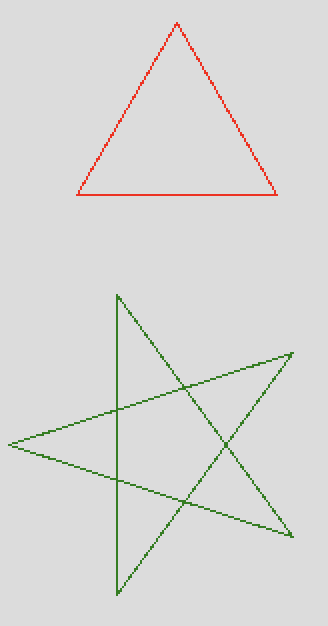
\includegraphics[width=\textwidth]{../images/turtle0.png}

\end{minipage}

\end{footnotesize}
\end{frame}


\begin{frame}[fragile]
\begin{footnotesize}

  \head{Fortolkning af Skildpaddekommandoer}
  \vspace{1ex}

  Før vi kan skrive en ``skildpaddekommandofortolker'' må vi først
  bestemme os for hvilke tilstande en skildpadde kan være i.

  \vspace{1ex}

  \head{Skildpaddetilstande:}
  \vspace{1ex}
  \begin{itemize}
  \item Position (type \lstinline{point = int*int}; initielt i midten af billedet)
  \item Retning (grader relativt til x-aksen: initielt $^\mathrm{o}$90).
  \item Farve (initielt sort på grå baggrund)
  \item Er pennen oppe eller nede (boolean; \lstinline{true} hvis oppe)
  \end{itemize}

  \vspace{1ex}
  Vi skal også bestemme os for hvad resultatet af ``fortolkningen'' skal være.
  \vspace{1ex}

  Hvis vi nu kunne fortolke kommandoerne til en \textbf{liste af
  linier} (af type \lstinline{point*point*color}) vil vi kunne benytte os af
  \lstinline{ImgUtil.setLine} til at tegne linierne på et bitmap:
\begin{lstlisting}[numbers=none,frame=none,mathescape]
val setLine : color -> int*int -> int*int -> bitmap -> unit
\end{lstlisting}

\end{footnotesize}
\end{frame}

\begin{frame}[fragile]
\begin{footnotesize}

  \head{Skildpaddekommandofortolkningen}
  \vspace{1ex}
\begin{lstlisting}[numbers=none,frame=none,mathescape]
type point = int * int
type line = point * point * color
let rec interp (p:point,d:int,c:color,up:bool) (cmds:cmd list) : line list =
  match cmds with
    | [] -> []
    | SetColor c :: cmds -> interp (p,d,c,up) cmds
    | Turn i :: cmds -> interp (p,d-i,c,up) cmds
    | PenUp :: cmds -> interp (p,d,c,true) cmds
    | PenDown :: cmds -> interp (p,d,c,false) cmds
    | Move i :: cmds ->
      let r = 2.0 * System.Math.PI * float d / 360.0
      let dx = int(float i * cos r)
      let dy = -int(float i * sin r)
      let (x,y) = p
      let p2 = (x+dx,y+dy)
      let lines = interp (p2,d,c,up) cmds
      if up then lines else (p,p2,c)::lines
\end{lstlisting}

\vspace{-25mm}\hspace{90mm}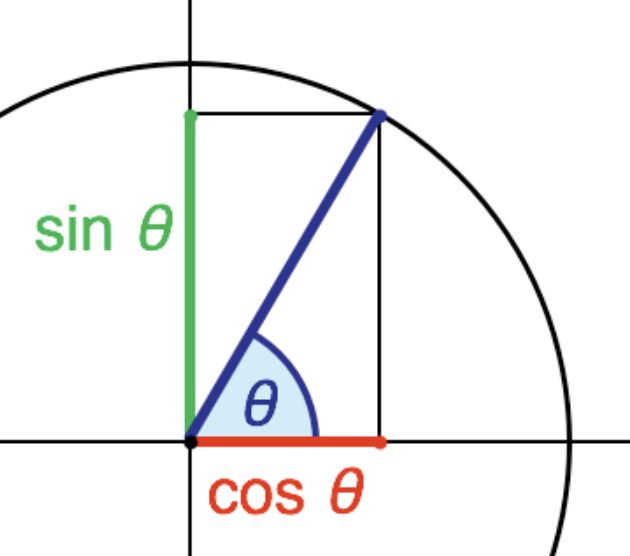
\includegraphics[width=25mm]{../images/cossin.png}

\end{footnotesize}
\end{frame}

\begin{frame}[fragile]
\begin{footnotesize}

  \head{Koden der tegner billedet og viser det i et vindue}
  \vspace{1ex}

\begin{lstlisting}[numbers=none,frame=none,mathescape]
let black = ImgUtil.fromRgb (0,0,0)

let draw (w,h) (pic: cmd list) =
  let C = ImgUtil.mk w h
  let center = (w/2, h/2)
  let dir_up = 90
  let initState = (center,dir_up,black,false)
  let lines = interp initState pic           // run interp
  for (p1,p2,c) in lines do
    ImgUtil.setLine c p1 p2 C                // update canvas
  ImgUtil.show "Logo" C                      // show canvas
\end{lstlisting}

  \head{Bemærk:}
  \begin{itemize}
  \item Vi benytter os af \lstinline{ImgUtil.mk} til at initialisere baggrunden.
  \item Vi benytter en for-in løkke samt
    \lstinline{setLine} til at tegne linierne på canvas'et.
  \end{itemize}

\end{footnotesize}
\end{frame}

\begin{frame}[fragile]
\begin{footnotesize}

  \head{Træ-fraktalen med skildpaddegrafik}
  \vspace{1ex}

\begin{minipage}{0.68\textwidth}

\begin{lstlisting}[numbers=none,frame=none,mathescape]
let rec tree sz =
  if sz < 5 then
    [Move sz; PenUp; Move (-sz); PenDown]
  else
    [Move (sz/3);
     Turn -30] @ tree (sz*2/3) @ [Turn 30;
     Move (sz/6);
     Turn 25] @ tree (sz/2) @ [Turn -25;
     Move (sz/3);
     Turn 25] @ tree (sz/2) @ [Turn -25;
     Move (sz/6); PenUp;
     Move (-sz/3);   // not safe to
     Move (-sz/6);   // reduce these
     Move (-sz/3);   // moves to a
     Move (-sz/6);   // single move!
     PenDown]
\end{lstlisting}
\end{minipage}
\begin{minipage}{0.3\textwidth}

  ~\hspace{-5mm}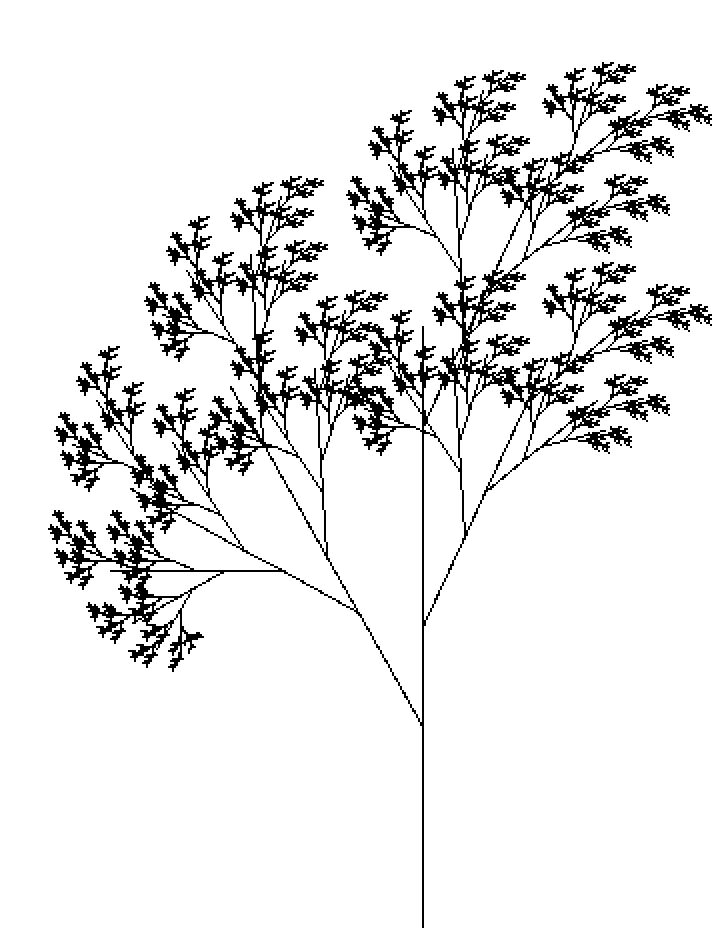
\includegraphics[width=1.2\textwidth]{../images/tree.png}

\end{minipage}

\vspace{1ex}
\textbf{Spørgsmål:} Hvorfor er det ikke en god ide at reducere de sidste fire
    \lstinline{Move} kommandoer til en enkelt \lstinline{Move}
    kommando?

\end{footnotesize}
\end{frame}

\begin{frame}[fragile]
\begin{footnotesize}

  \headsp{Oversættelse og kørsel med \lstinline{img_util.dll}}

Følgende kommando bruges til at konstruere \lstinline{img_util.dll} - under macOS:

\begin{tiny}
\begin{verbatim}
  $ fsharpc --nologo \
     -I /Library/Frameworks/Mono.framework/Versions/Current/lib/mono/gtk-sharp-2.0 \
     -r gdk-sharp.dll -r gtk-sharp.dll -a img_util.fsi img_util.fs
\end{verbatim}
\end{tiny}

\vspace{3mm}

\begin{minipage}{.72\textwidth}
Oversættelse og kørsel af \lstinline{turtle.fs}:

\begin{verbatim}
  $ fsharpc --nologo -r img_util.dll turtle.fs
  $ mono turtle.exe
\end{verbatim}

\vspace{2mm}

\textbf{Bemærk:}

\begin{itemize}
\item Kopier eventuelt \lstinline{img_util.dll} til src-biblioteket.
  \item Se \url{https://github.com/diku-dk/img-util-fs} for
detaljer om kørsel på Windows 10 og Linux.
\end{itemize}
\end{minipage}\hfill
\begin{minipage}{.25\textwidth}
  \vspace{0pt}
  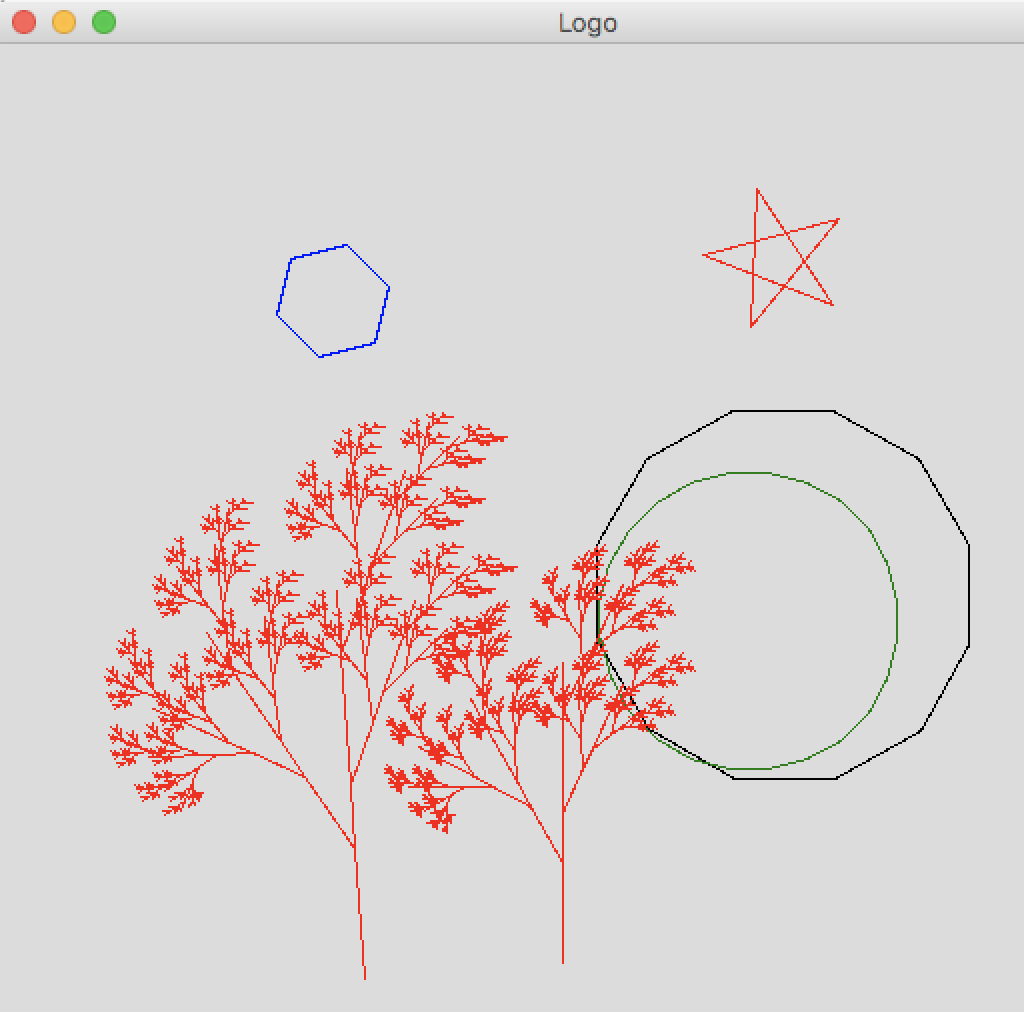
\includegraphics[width=.9\textwidth]{../images/turtle.png}
\end{minipage}

\end{footnotesize}
\end{frame}


\subsection{Abstrakte typer med moduler}

\begin{frame}[fragile]
\begin{footnotesize}

  \headsp{Abstrakte typer med moduler}

  \begin{quote}Moduler kan benyttes til at \emph{indkapsle} en type sammen med operationer på typen.
  \end{quote}

  \vspace{2mm}
\begin{minipage}[t]{0.53\textwidth}
  \vspace{0pt}
  \headsp{To eksempler: Stakke og køer}

    To data-strukturer der let kan implementeres med lister og
    mønstergenkendelse og hvis implementation og repræsentation kan
    holdes abstrakt (dvs. skjult) ved brug af \textbf{abstrakte modul typer}.
\end{minipage}
\hfill
\begin{minipage}[t]{0.4\textwidth}
  \vspace{0pt}
  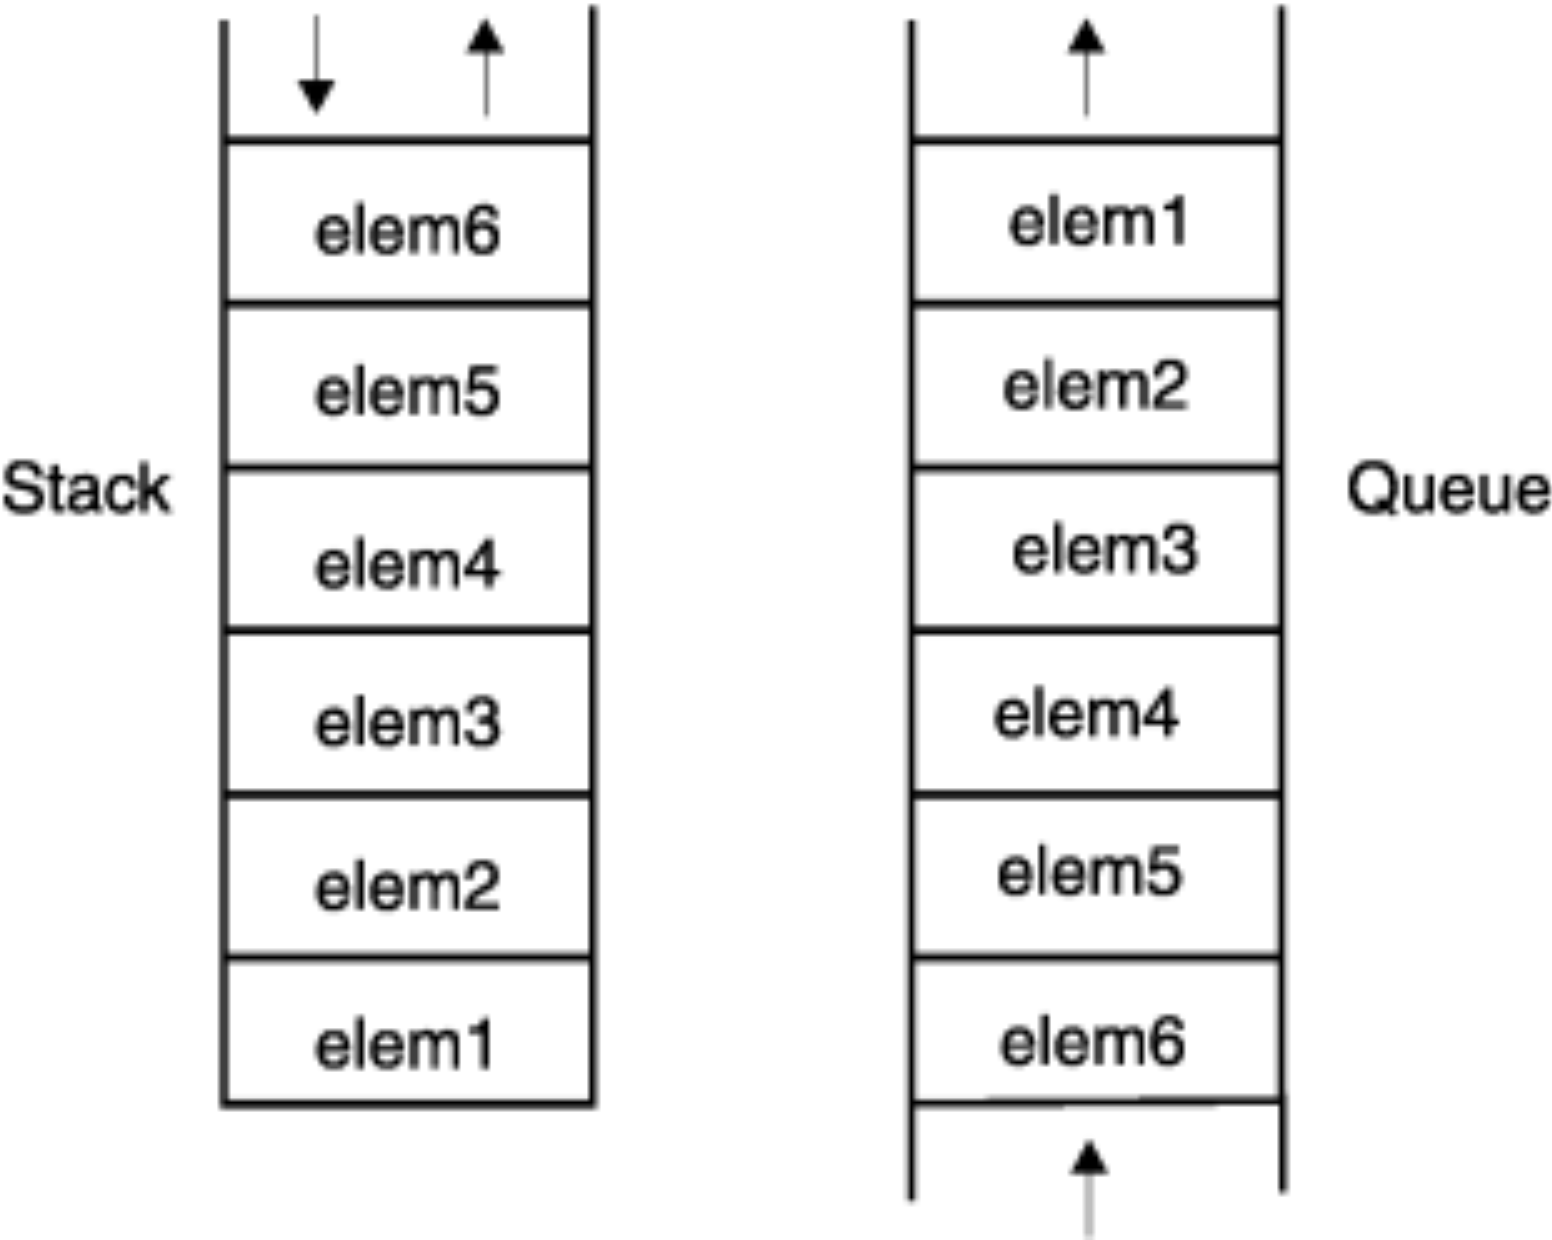
\includegraphics[width=\textwidth]{../images/lifofifo.png}
\end{minipage}
\end{footnotesize}
\end{frame}

\subsection{Eksempel: Stakke}

\begin{frame}[fragile]
\begin{footnotesize}

  \head{Eksempel: Stakke}

  \vspace{1ex}

\begin{minipage}[b]{0.80\textwidth}

  En \emph{stak} er en data-struktur med et simpelt interface:

  \vspace{1ex}

\begin{lstlisting}[numbers=none,frame=none,mathescape]
module Stack // content of stack.fsi

type 'a stack                          // LIFO
val empty : unit -> 'a stack
val push  : 'a stack -> 'a -> 'a stack
val pop   : 'a stack -> ('a * 'a stack) option
\end{lstlisting}
  \vspace{1ex}
  \head{Spørgsmål:}
\begin{itemize}
\item Hvordan implementeres et stak-modul?
\item Hvordan sikres det at man \textbf{KUN} kan tilgå værdier af type
  \lstinline{'a stack} med operationerne \lstinline{pop} og
  \lstinline{push}?
\end{itemize}

\end{minipage} \hspace{-8mm}
\begin{minipage}[b]{0.16\textwidth}

  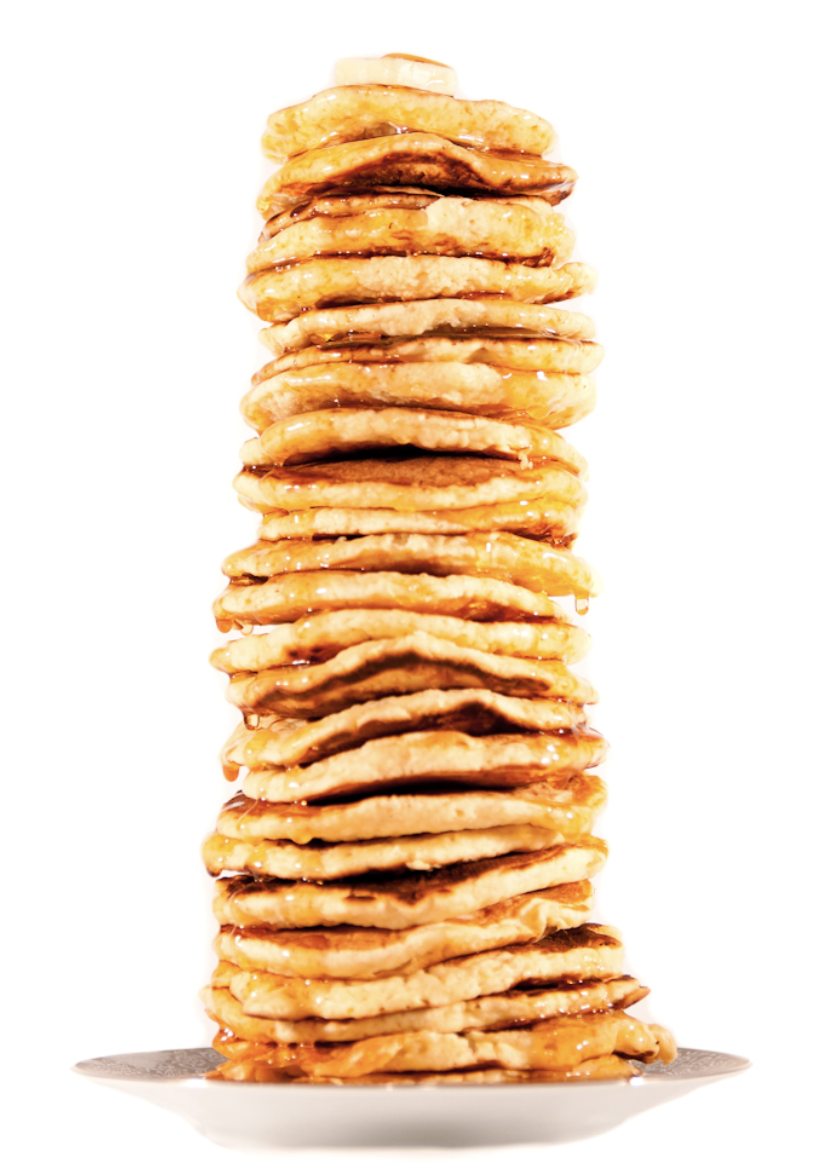
\includegraphics[width=1.8\textwidth]{../images/stack.png}

\end{minipage}

\end{footnotesize}
\end{frame}

\begin{frame}[fragile]
\begin{footnotesize}

  \head{Stak-implementation}

  \vspace{1ex}


\begin{lstlisting}[numbers=none,frame=none,mathescape]
module Stack

type 'a stack = S of 'a list
let empty () = S []
let push (S s: 'a stack) v = S (v::s)
let pop (S s) : ('a * 'a stack) option =
  match s with
    | [] -> None
    | x::xs -> Some (x,S xs)
\end{lstlisting}

  \vspace{1ex}
  \head{Bemærk:}
\begin{itemize}
\item Enkel version ved brug af \lstinline{'a list}.
\item Singleton ``Sum-type'' benyttes til at sikre \textbf{fuld abstraktion} (\lstinline{S} konstruktør) .
\item Modul skal oversættes med både fsi-fil og fs-fil:
\begin{verbatim}
$ fsharpc -a stack.fsi stack.fs
$ fsharpi -r stack.dll
\end{verbatim}
\end{itemize}

\end{footnotesize}
\end{frame}

\subsection{Eksempel: Køer}

\begin{frame}[fragile]
\begin{footnotesize}

  \head{Eksempel: Køer}

  \vspace{1ex}

\begin{minipage}[b]{0.80\textwidth}

  En \emph{kø} er en data-struktur med et simpelt interface:

  \vspace{1ex}

\begin{lstlisting}[numbers=none,frame=none,mathescape]
module Queue // content of queue.fsi

type 'a queue                        // FIFO
val empty : unit -> 'a queue
val insert  : 'a queue -> 'a -> 'a queue
val remove  : 'a queue -> ('a * 'a queue) option
\end{lstlisting}
  \vspace{1ex}
  \head{Spørgsmål:}
\begin{itemize}
\item Hvordan implementers et kø-modul?
\item Hvordan sikres det at man \textbf{KUN} kan tilgå værdier af type
  \lstinline{'a queue} med operationerne \lstinline{insert} og
  \lstinline{remove}?
\end{itemize}

\end{minipage} \hspace{-4mm}
\begin{minipage}[b]{0.16\textwidth}

  
\includegraphics[width=1.4\textwidth,height=3cm]{../images/queue.png}

\end{minipage}

\end{footnotesize}
\end{frame}

\begin{frame}[fragile]
\begin{footnotesize}

  \head{Kø-implementation --- NOT GOOD --- file \texttt{queue\_bad.fs}}

  \vspace{1ex}

\begin{lstlisting}[numbers=none,frame=none,mathescape]
module Queue

type 'a queue = Q of 'a list                 // BAD
let empty () = Q []                          // BAD
let insert (Q q: 'a queue) v = Q (v::s)      // BAD
let remove (Q q) : ('a * 'a queue) option =  // BAD
  match List.rev q with                      // BAD
    | [] -> None                             // BAD
    | x::xs -> Some (x,Q (List.rev xs))      // BAD
\end{lstlisting}

  \vspace{1ex}
  \head{Bemærk:}
\begin{itemize}
\item Enkel version ved brug af \lstinline{'a list}.
\item Singleton ``Sum-type'' benyttes til at sikre \textbf{fuld abstraktion} (\lstinline{Q} konstruktør) .
\end{itemize}

  \vspace{1ex}
  \head{Spørgsmål:}
  \begin{itemize}
  \item Hvad er problemet?
\end{itemize}

\end{footnotesize}
\end{frame}

\begin{frame}[fragile]
\begin{footnotesize}

  \head{Kø-test --- file \texttt{qtest.fs}}

  \vspace{1ex}

\begin{lstlisting}[numbers=none,frame=none,mathescape]
  module Q = Queue
  let q = List.fold (fun q v -> Q.insert q v) (Q.empty()) [0..5000]
  let rec loop q = match Q.remove q with
                     | None -> 0
                     | Some (v,q) -> v + loop q
  let a = loop q
  do printfn "sum(queue) = %d" a
\end{lstlisting}

  \vspace{1ex}

\head{Kørsel med \texttt{queue\_bad.fs}}
\begin{verbatim}
cp queue_bad.fs queue.fs
fsharpc --nologo -a queue.fsi queue.fs
fsharpc --nologo -r queue.dll qtest.fs
time mono qtest.exe
sum(queue) = 12502500
        3.60 real         4.12 user         0.14 sys
\end{verbatim}
\end{footnotesize}
\end{frame}

\begin{frame}[fragile]
\begin{footnotesize}

  \head{En bedre kø-implementation --- file \texttt{queue\_good.fs}}

  \vspace{1ex}

\begin{lstlisting}[numbers=none,frame=none,mathescape]
module Queue     // GOOD Queue Implementation

type 'a queue = Q of 'a list * 'a list
let empty () = Q ([],[])
let insert (Q (b,f)) v = Q (v::b,f)
let remove (Q (b,f)) : ('a * 'a queue) option =
  match f with
    | x :: xs -> Some (x,Q(b,xs))
    | [] ->
      match List.rev b with
        | [] -> None
        | x :: xs -> Some (x,Q([],xs))
\end{lstlisting}

  \vspace{1ex}
  \head{Bemærk:}
\begin{itemize}
\item To lister: en til ``indsættelse'' og en til ``fjernelse''.
\item Hvis listen til fjernelse er tom tages hele listen til
  indsættelse og indsættes i listen til fjernelse (efter at den er
  vendt om).
\end{itemize}

\end{footnotesize}
\end{frame}

\begin{frame}[fragile]
\begin{footnotesize}

\head{Kørsel af \texttt{qtest.fs} med \texttt{queue\_good.fs}}
  \vspace{1ex}

\begin{verbatim}
cp queue_good.fs queue.fs
fsharpc --nologo -a queue.fsi queue.fs
fsharpc --nologo -r queue.dll qtest.fs
time mono qtest.exe
sum(queue) = 12502500
        0.06 real         0.04 user         0.00 sys
\end{verbatim}

  \vspace{1ex}
  \head{Bemærk:}
\begin{itemize}
\item Vi har formået at ændre implementationen af kø-modulet uden at programmet \texttt{qtest.fs} kan ``se forskel''.
\item Applikationen virker stadig korrekt (hvilket kunne testes med black-box unit testing).
\item Effekten er blot at programmet \texttt{qtest.fs} nu kører hurtigere!

  (Før 3 sekunder nu 60 millisekunder...)
\end{itemize}

\end{footnotesize}
\end{frame}

\subsection*{Konklusion}
\begin{frame}[fragile]
  \headsp{Konklusion}

  \vspace{3mm}
  \tableofcontents
\end{frame}

\end{document}
